\documentclass[tikz,border=10pt]{standalone}
\begin{document}
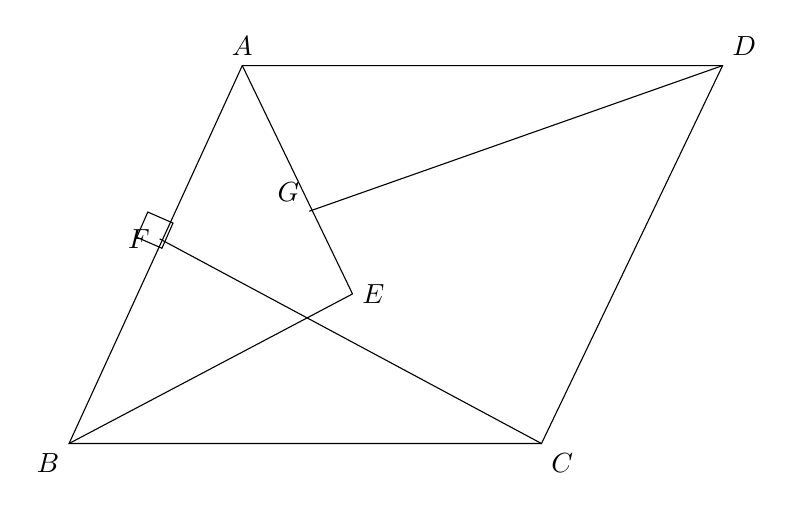
\begin{tikzpicture}[scale=1]

% Coordinates
\coordinate (B) at (0,0);
\coordinate (C) at (6,0);
\coordinate (D) at (8.3,4.8);
\coordinate (A) at (2.2,4.8);

\coordinate (E) at (3.6,1.9);
\coordinate (F) at (1.15,2.6);
\coordinate (G) at (3.05,2.95);

% Outer parallelogram
\draw (A) -- (D) -- (C) -- (B) -- cycle;

% Interior segments
\draw (A) -- (E);
\draw (B) -- (E);
\draw (F) -- (C);
\draw (G) -- (D);

% Right-angle mark at F between AB and FC
\draw (1.18,2.48) -- (1.32,2.80) -- (1.00,2.94) -- (0.86,2.62) -- cycle;

% Labels
\node[above] at (A) {$A$};
\node[below left] at (B) {$B$};
\node[below right] at (C) {$C$};
\node[above right] at (D) {$D$};
\node[left] at (F) {$F$};
\node[right] at (E) {$E$};
\node[above left] at (G) {$G$};

\end{tikzpicture}
\end{document}
